% !TEX encoding = UTF-8 Unicode
% !TEX root = ../../Masterthesis.tex

\chapter{Star Trek}\label{ch:star trek}

\begin{center}
\textit{Space: the final frontier. \\ These are the voyages of the starship Enterprise. Its continuing mission: \\ to explore strange new worlds, to seek out new life and new civilizations, \\ to boldly go where no one has gone before.}
\end{center}
\begin{flushright}
--- As narrated by Captain. Jean-Luc Picard \\
\parencite{day_boldly_2005}
\end{flushright}

%-----------------------------------------------------------------------------
% These Are The Voyages...
%-----------------------------------------------------------------------------

\section{These Are The Voyages...}

\begin{figure}
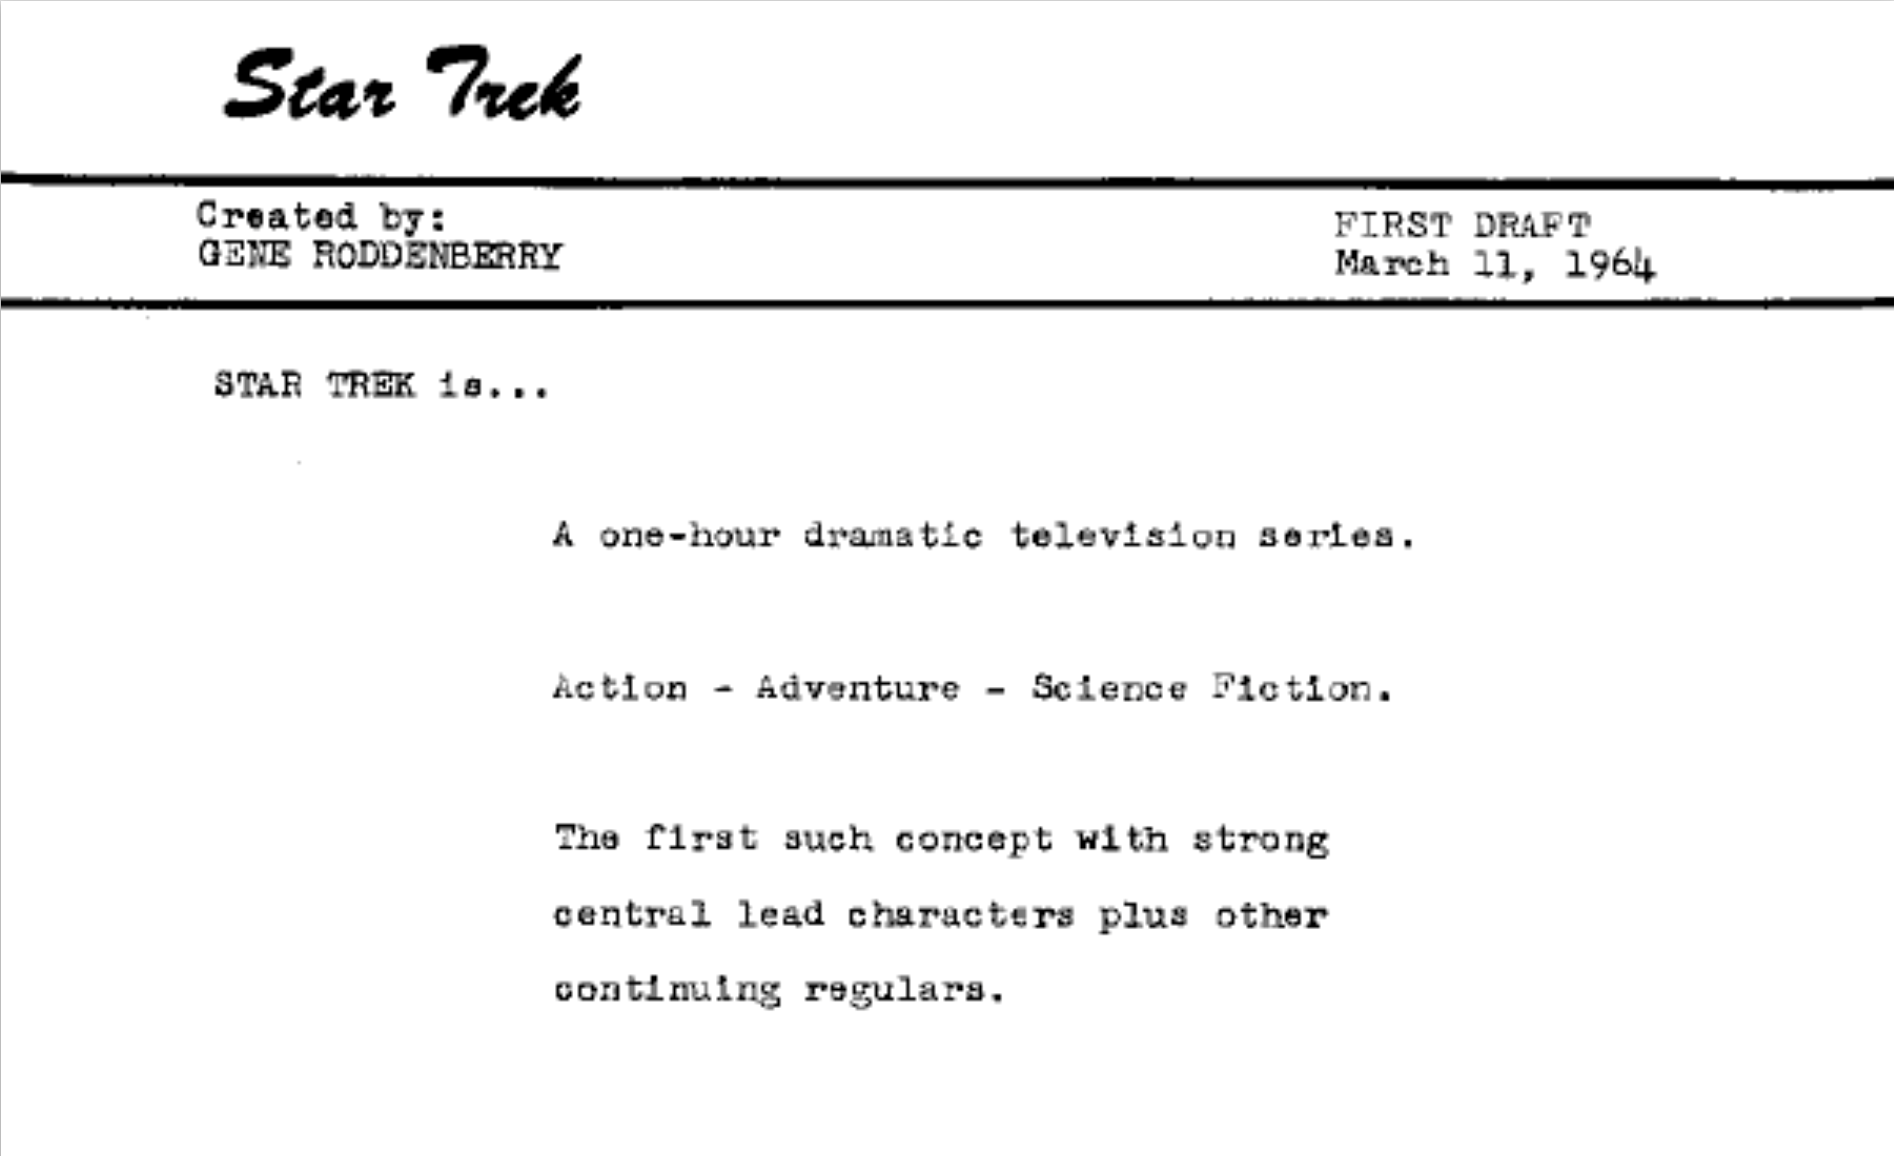
\includegraphics[width=\linewidth]{star_strek_roddenberry_pitch}
\caption{Gene Roddenberry's original pitch for Star Trek to NBC}
\end{figure}

\newthought{Star Trek is an} American science fiction TV and motion picture franchise, created by \textit{Gene Roddenberry}. It debuted with the pilot ``The Cage'' in 1966 on NBC and has since evolved into hundreds of books and novels, several computer games, six TV series\footnote{See table \ref{tb:tv series}}, and twelve motion pictures\footnote{See table \ref{tb:filmography}}. The basic premise of the show is an interstellar adventure in the beginning of the 23rd century where we follow the actions of the captains and crew on the starship Enterprise.\footnote{Except DS9 which takes place on a space station rather then a starship.} They follow the orders of \textit{Starfleet}, which is the scientific and exploratory branch of \textit{The United Federation of Planets}, a multi-planetary alliance. Star Trek displays a rather philanthropic view on the human race. The economy has moved away from capitalism, the crime rate is essentially zero and religion is essentially obsolete. According to Roddenberry, humans in the 23rd century are,
\blockquote[{\cite{roddenberry_star_1987}}]
{
(...)intelligent, witty, thoughtful, compassionate, caring (...) -- but they have human faults and weaknesses too -- although not as many or as severe as in our time. (...)The major problems facing the human species have been resolved and the Earth has since been transformed into a human paradise.
}
The crew on the Enterprise consists of both humans and aliens, and the hierarchy and terminology used is in direct parallel with the Navy: they have ranks like Chief Petty Officer, Ensign, Captain, and Admiral and they use terms like ``port'' and ``starboard'' and the bridge is the main control room.

\begin{margintable}
\small
\begin{tabular}{ll}
\toprule
	\textbf{TV-show}		& \textbf{Running}	\\
\midrule
    	The Original Series		& 1966-1969		\\
        The Animated Series		& 1973-1974		\\
        The Next Generation 	& 1987-1994		\\
        Deep Space Nine 		& 1993-1999		\\
        Voyager					& 1995-2001		\\
        Enterprise				& 2001-2005		\\
\bottomrule
\end{tabular}
	\caption{Star Trek TV series}
	\label{tb:tv series}
\end{margintable}

While Star Trek is widely regarded as a successful franchise, it had a rough start. \textit{The Original Series} ran for only three years. Even though the fan base was substantial, ever increasing budget cuts and tighter time schedules caused the show to finally call it quits in 1969. It would be 10 years before Paramount dared commit to a large scale motion picture. \parencite[87]{bond_music_1998}


%-----------------------------------------------------------------------------
% The Music of Star Trek
%-----------------------------------------------------------------------------

\begin{figure}
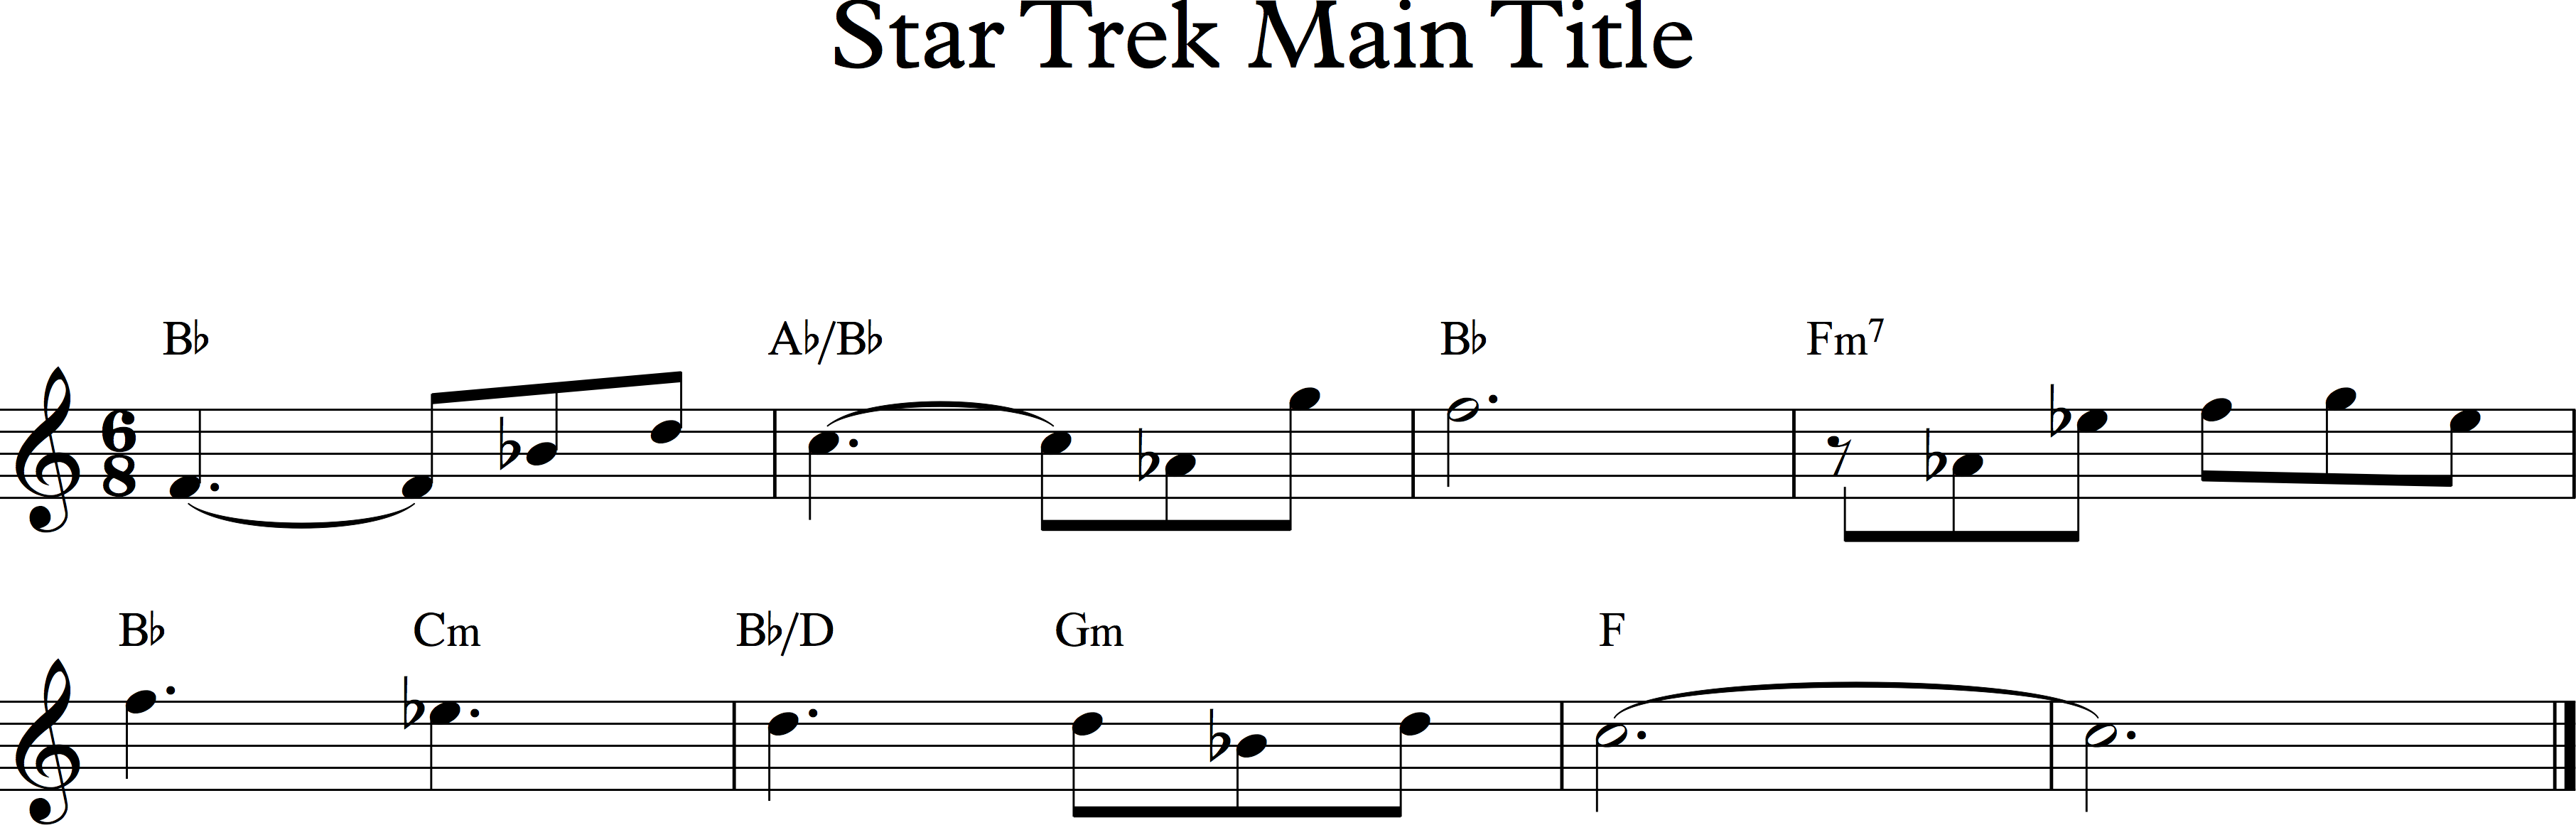
\includegraphics[width=\linewidth]{gfx/snippet_main_theme}
\caption{Goldsmith's ``Star Trek Theme''}
\end{figure}

\section{The Music of Star Trek}

\marginnote{\textbf{Jerry Goldsmith} selected filmography:
\begin{itemize}
\item Planet of the Apes (1968)
\item The Omen (1976)
\item Alien (1979)
\item Poltergeist (1982)
\item First Blood (1982)
\item Twilight Zone: The Movie (1983)
\item Total Recall (1990)
\item Basic Instinct (1992)
\item Mulan (1998)
\end{itemize}
}
Much like the Super Mario theme, the Star Trek theme is nearly ubiquitous in pop culture and is immediately recognized by most. In fact, Star Trek catch phrases have taken root in english vernacular. There are few that have not heard the phrase ``Beam me up, Scotty!'' or ``Damn it man. I'm a doctor, not a [\ldots]''. With similar influence, the music of Star Trek has pioneered what the ``future'' sounds like. The first Star Trek movie: \ac{ST:TMP}, directed by \textit{Robert Wise}, was planed as early as 1973, but Paramount did not have the confidence to finance an expensive and risky production. It was not until \textit{George Lucas}' space epic \textit{Star Wars (1977)}, scored by \textit{John Williams}, hit the theaters to enormous applause that Paramount gave \ac{ST:TMP} the green light \parencite{bond_music_1998}. \textit{The Original Series} had new music written for every episode, bearing the signature of some of the all time greatest composers in Hollywood\footnote{See table \ref{tb:star trek composers}}. However, when choosing who would compose the very first Star Trek motion picture, Paramount looked for a composer that could match the epic score of John Williams. \textit{Jerry Goldsmith (1929-2004)} had just finished the acclaimed 20th Century Fox production \textit{Alien (1979)} and had scored several science fiction blockbusters already, making him the perfect candidate \parencite[87]{bond_music_1998}.

Much of the stylistic elements in \ac{ST:TMP} are borderline avant-garde and full of romantic elements. Goldsmith utilizes synthesizers, church organs, and a custom made instrument called ``Blaster Beam''.\footnote{
A musical instrument refined and made famous by Craig Huxley.
}
Some of the movie scenes are fairly long making some of the musical cues fairly long as well. Goldsmith utilizes this by building cues matching the slow tempo and thus bringing more traditional compositional couplings into the cue. In \nameref{sec:leaving drydock} (analyzed on p.~\pageref{sec:leaving drydock}) we see a cue 3:32 minutes long accompanying ``The drydock sequence''. Jeff Bond notes the following: \blockquote[{\cite[88]{bond_music_1998}}]
{
Maintaining interest in the scene was a task that mainly fell to Goldsmith, and the challenge resulted in a pice of music with an unusual amount of classical development and structure, a hallmark of Goldsmiths's epic style of the late `70s and early `80s.
}
The now famous march Goldsmith composed later became the title track for the TV-series \textit{``The Next Generation''} making it what we could call the ``Star Trek Theme''.

\begin{table*}
\small
\begin{tabularx}{\linewidth}{p{5.2cm} p{3.2cm} l l}
		\multicolumn{4}{c}{Star Trek, movies and composers}\\
\toprule
		\textbf{Film} 					& \textbf{Composers}		& \textbf{Date Released}	& \textbf{Series}		\\
\midrule
		Star Trek: The Motion Picture		& Jerry Goldsmith			& 1979, 7 December 	& The Original Series 	\\
		ST II: The Wrath of Khan  			& James Horner				& 1982, 4 June  		& 					\\
		ST III: The Search for Spock  		& James Horner				& 1984, 1 June 			&  					\\
		ST IV: The Voyage Home				& Leonard Rosenman			& 1986, 26 November 	&  					\\
		ST V: The Final Frontier			& Jerry Goldsmith			& 1989, 9 June 			&  					\\
		ST VI: The Undiscovered Country		& Cliff Eidelman			& 1991, 6 December		&  					\\
		ST VII: Generations					& Dennis McCarthy			& 1994, 18 November		& The Next Generation	\\
		ST VIII: First Contact  			& Jerry Goldsmith\(\dagger\)& 1996, 22 November		&  					\\
		ST IX: Insurrection    				& Jerry Goldsmith			& 1998, 11 December		&  					\\
		ST X: Nemesis     					& Jerry Goldsmith			& 2002, 13 December		&  					\\
		Star Trek XI     					& Michael Giacchino			& 2009, 8 May			& Reboot Cast			\\
		ST XII: Into Darkness  				& Michael Giacchino			& 2013, 16 May			& 					\\
\bottomrule
    \(\dagger\) With his son Joel Goldsmith	&							&					&					\\
\end{tabularx}
    \caption{Star Trek filmography}
    \label{tb:filmography}
\end{table*}

\marginnote[2cm]{\textbf{James Horner} selected filmography:
\begin{itemize}
\item Aliens (1986)
\item Honey, I Shrunk the Kids (1989)
\item Searching for Bobby Fischer (1993)
\item Braveheart (1995)
\item Apollo 13 (1995)
\item Titanic (1997)
\item Avatar (2009)
\item The Karate Kid (2010)
\end{itemize}}

\textbf{Star Trek II: The Wrath of Khan} was \textit{James Horner's (1953-2015)} big breakthrough as a feature film composer. The main reason Goldsmith was not utilized for this offering was budget cuts, making Horner -the ``new guy''- much cheaper to hire. Horner had scored a number of low-budget science fiction films previously, like \textit{``Humanoids From the Deep''} and \textit{''Battle Beyond the Stars''}, which incidentally has a striking similarity to the Star Trek II score.

The overall tone of the score owes much to Goldsmith and Williams; however, the score is manifestly Horneresque. The score is well loved by fans and critiques, despite the poor orchestral performance, which is under balanced and poorly executed.

Although not part of my thesis as such, it is worth noting some of the quite serious critique Horner has received for his compositional works. He is one of the most used composers in Hollywood but he has had to endure a lot of critique over the years for plagiarism. The case of artists ``borrowing'' from one another is not new and perhaps is impossible to avoid. The TED talk ``Embrace the Remix'' \footnote{\textcite{Ferguson2012}} discusses this phenomenon thoroughly. I believe no motif can be copyrighted as such, but they are part of a composers signature. In Horner's case the evidence would suggest that he not only borrows motives and harmonic progressions, but also references entire passages without giving credit to the original composer, like \textit{Sergei Prokofiev's - Alexander Nevsky: part 5}, which he references extensively in both his Star Trek scores, and Sergei Rachmaninov's theme from his first symphony. It is also very clear that he reuses his own material quite frequently, like the example mention earlier in which the similarity between \textit{``Battle Beyond the Stars''} main title and the main title of \textbf{Star Trek II} are quite striking.

\begin{marginfigure}
\center
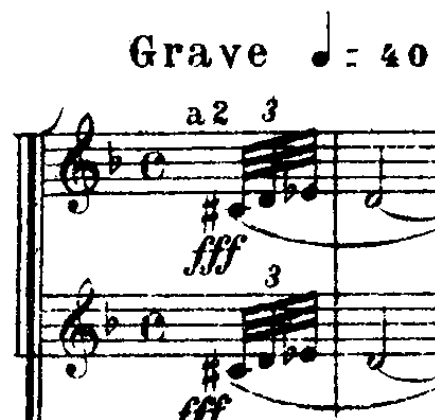
\includegraphics[width=0.7\linewidth]{rach_danger_motiv}
	\caption[Rachmaninov's 1st Symphony]{Snippet from the first bar of Rachmaninov's 1st Symphony. Exactly the same as Horner's ``Danger Theme'' which he has used throughout his career, and notedly in \textbf{Star Trek II}: ``Surprise Attack''}
	\label{fg:danger theme}
\end{marginfigure}

\textbf{Star Trek: First Contact} was directed by Star Trek actor \textit{Jonathan Frakes}, released in 1996 and was subject to high expectations because the previous \textbf{Star Trek: Generations} had been less of a success. While the overall looks of \textbf{Generations} was beautiful, the story had several weak points and distanced it self from the audience. The music got negative critique as well: \blockquote[{\cite[152]{bond_music_1998}}]
{MacCarthy's overture theme was memorable and his Nexus music quite beautiful, but the lack of repeated motifs and melodies in many of the other scenes lent a somewhat disconnected quality to the score as a whole.}
The pressure was therefor on to remedy the damage done. Jerry Goldsmith was hired to do the job, but because of time pressure Goldsmith hired his son, \textit{Joel Goldsmith} to do the majority of action cues for the score. Joel produced total of 22 minutes of music for \textbf{First Contact}.

\marginnote[-3cm]{\textbf{Michael Giacchino} selected filmography:
\begin{itemize}
\item Medal of Honor: Underground (2000)
\item The Incredibles (2004)
\item Lost (2004)
\item Mission: Impossible III (2006)
\item Ratatouille (2007)
\item Up (2009)
\item Dawn of the Planet of the Apes (2014)
\end{itemize}}

\textbf{Star Trek: Nemesis} was the tenth, and last in the line of Star Trek films for some years to come. It was the third film featuring the cast of \textbf{The Next Generation} and was the mark of the end of an era. It was directed by \textit{Stuart Baird} and was released in 2002. Jerry Goldsmith was hired to score \textbf{Nemesis}, his fifth Star Trek movie (see figure \ref{fg:st composers}) and had long since become synonymous with the music of Star Trek \parencite{bond_2013}. Much of the score focuses on \textit{Shinzon's theme} (see figure \ref{shinzons_theme}), the main antagonist. Goldsmith treats his theme through several variations throughout the score\footnote{Hint's of it may be heard at the end of the main title \textit{Remus} and first heard clearly in the second half of \textit{Positronic Signal.}}. Goldsmith revisits themes from his past Star Trek movies in bits and pieces throughout, they are after all an important part of Star Trek lore, but he also created new themes that stand out as highlights of the movie. Like the new, heroic march in \textit{Battle Stations} \textquote[{\cite[215]{bond_2013}}]{(\ldots)that encapsulates Picard's sense of duty and his inherent nobility perfectly.}

\begin{marginfigure}
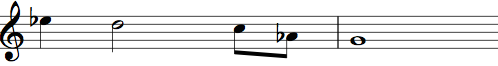
\includegraphics[width=\linewidth]{shinzons_theme}
	\caption{Part of Shinzon's Theme}
	\label{shinzons_theme}
\end{marginfigure}

In 2009 \textbf{Star Trek}, directed by \textit{J.J. Abrams}, came to cinemas across the world. Michael Giacchino, a regular collaborator of Abrams', was to pick up the mantle after Goldsmith. With almost 30 years of Star Trek history, expectations for Giacchino's score was high. The score turned out to strike out in a new branch leaving the old thematic material behind for a new, omnipresent theme Giacchino uses in virtually every major cue. All over, Giacchino's score use a simpler harmonic language, and lacks the ``sci-fi adventure'' found in Goldsmith and Horner's Star Trek scores. \textbf{Star Trek} did suffer from post production difficulties regarding the sound FX and music. The music got reworked extensively on the cutting floor, making analyzing the music from the source harder, due to the layers of dialogue and special-effects.
\footnote{
\textquote[\cite{takis_score_2010}]{In some cases, cues that had been displaced from their intended positions were replaced or supplemented by editorial creations.}
}
Fortunately a ``Deluxe'' edition CD was released which figured many of the original, unaltered cues. This, combined with the altered cues we hear in the movie score, gives us a reasonable view of the overall sonority.

\textbf{Star Trek: Into Darkness} is the second of the rebooted series, and was released in 2013 with J.J. Abrams and Giacchino at the helm. Now a defined part of something new, the sweeping romantic grandeur from Goldsmith's time is part of the \textit{Ars Antiqua}. Apart from the overall flattened harmonic complexity the score suffers from a low and lifeless mix in the final movie. Nevertheless, the score is more intricate than the 2009 movie and shows that Giacchino now had the time to evolve the sound and adapt it to the new universe.

\begin{table*}
\small
\begin{tabularx}{\linewidth}{lllX}
\toprule
	\textbf{Composer}	& \textbf{Movie score} 				& \textbf{Series theme} 			& \textbf{Incidental music} \\
\midrule
	Alexander Courage 	& 								& The Original Series 			& The Original Series \\
	Cliff Eidelman 		& ST VI: The Undiscovered Country 		&  							&  \\
	David Bell			&  								&  							& Deep Space Nine, Voyager, Enterprise \\
	Dennis McCarthy 	& ST VII Generations 				& Deep Space Nine 				& The Next Generation, Deep Space Nine, Voyager, Enterprise \\
	Diane Warren 		&  								& Enterprise 					&  \\
	Fred Steiner 		&  								&  							& The Original Series, The Next Generation \\
	George Duning 	&  								&  							& The Original Series \\
	Gerald Fried 		& 								&  							& The Original Series \\
	James Horner 		& ST II: The Wrath of Khan			&  							&  \\
					& ST III: The Search for Spock 			&  							&  \\
	Jay Chattaway 		&  								& 							& The Next Generation, Deep Space Nine, Voyager, Enterprise  \\
	Jerry Goldsmith 	& ST: The Motion Picture				& The Next Generation   			&  \\
					& ST V: The Final Frontier				& Voyager						&  \\
					& ST VIII: First Contact				& 		 					&  \\
					& ST: IX Insurrection					&  							&  \\
					& ST X: Nemesis 					&  							&  \\
	Leonard Rosenman 	& ST IV: The Voyage Home 			&  							&  \\
	Michael Giacchino 	& Star Trek XI						&							&  \\
					& ST XII: into Darkness 				&  							&  \\
	Paul Baillargeon 	&  								& 							& Deep Space Nine, Voyager, Enterprise \\
	Ron Jones 		&  								&  							& The Next Generation \\
	Sol Kaplan 		&  								&  							& The Original Series \\
	Velton Ray Bunch 	&  								&  							& Enterprise \\
\bottomrule
\end{tabularx}
\caption{List of Star Trek composers}
\label{tb:star trek composers}
\end{table*}

% Reviewd jan 2016
